\subsection*{Network Metrics Analysis}
\addcontentsline{toc}{subsection}{Network Metrics Analysis}%
\subsubsection*{Modularity}
modularity equations\\
$Q = \frac {1} {4 m}\sum_ {ij} (A_{ij} - \frac {k_{i} k_{j}}{2 m}) \
s_{i} s_{j}$\\
$B_{ij} = A_{ij} - \frac {k_ {i} k_ {j}} {2 m}$\\
$Q = \frac {1} {4 m} s^{T} Bs = \frac {1} {4 m}\sum_ {i = 
	1}^{n} (u_ {i}^{T} . s)^{2}\beta_ {i}$\\
$\Delta Q = \frac {1} {4 m} s^{T} B^{(g)} s$\\
$B_{ij}^{(g)} = B_{ij} - \delta_{ij}\sum_ {k\in g} B_{ik}$

It is important to discuss how randomization has been done since the plot results can vary based on the generated null model via that specific randomization method. 
Random graphs were generated and below instruments were plotted.

Average degree vs time windows
Average betweenness centrality vs time windows
Modularity (Wolfram method) vs time windows
Modularity (GN method, algorithm by me) vs time windows
Average modularity for single random graph vs time windows
Z-scores for GN-modularity with Erdös-Renyi randomized null models vs time windows
Z-scores for GN-modularity randomized null models with fixed degree sequences vs time windows

Performing switch-randomization to a modular graph might fail even due to small details in randomization steps. That failure is probably the reason of high values of Z-scores in two different plots of Z-scores. If I try to switch randomize a modular graph, I could imagine a procedure where I take links only from same module and switch them or links that are across modules and switch them. And I mixed the sets of intra-module edges and inter-module edges separately. This null model might give a different result in Z-scores.

before treating time windows, having the modularity as function of bucket size and as function of step size. At this stage, choosing suitable step and bucket sizes and accordingly repeat all progress mentioned above. The aim is to obtain big amount of nodes as possible as we can and keeping that amount of nodes same in both graph structures (fixed step size and fixed bucket size). The difference between modularity values at highest graph nodes amount in fixed bucket and fixed step sized graphs shows which network structure is more effective on generating clear communities. In other words, modularity values is more meaningful when the node number is high.

Introduce hierarchical modularity and its relation with null models.

\subsubsection*{Different Types of Null Model}
Fixed Degree Sequence random graphs generation, a third one: Conserving Inter-edges and Intra-edges Among Modules random graphs were generated, accordingly, Z-scores were computed among those null models.

I have recomputed my constraint impact analysis pipeline for four production lines with re-defined null models: Degrees Fixed and Modularity and different choice of binning in terms of step-size \& bucket-size. The results are given in the attached PNG file.

Clarification of some details in the plot results as,
•	Please find below the cartoon showing how I generated the null models in a pairwise shuffling fashion to prevent ambiguity.

 \begin{figure}[!ht]
	\begin{center}
		\makebox[\textwidth]{
			\centering
			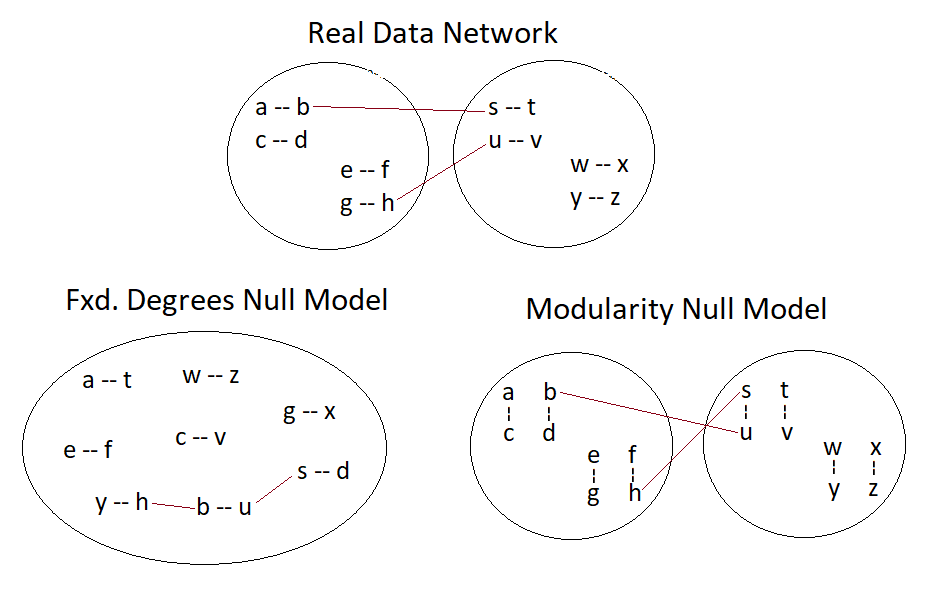
\includegraphics[width=0.6\linewidth]{../images/cartoon-null-model-definitions.png}}
		\caption{Formation of Different Null Models.}
		\label{figure-null_models}
	\end{center}
\end{figure}
\clearpage